% ===============================================================
% APRESENTAÇÃO FINAL - TCC2 - SENAC SANTO AMARO
% ===============================================================
% Versão enxuta e visual: textos resumidos em tópicos curtos
% e tamanhos de fonte ajustados para caber confortavelmente na tela.
% ===============================================================

\documentclass[
    aspectratio=169,
    11pt,
    brazil
]{beamer}

% ---------------------------------------------------------------
% PACOTES
% ---------------------------------------------------------------
\usepackage[brazil]{babel}
\usepackage{graphicx}
\usepackage{booktabs}
\usepackage{array}
\usepackage{tikz}
\usetikzlibrary{arrows.meta,positioning,fit,calc}
\usepackage{pgfplots}
\pgfplotsset{compat=1.18}
\usepgfplotslibrary{groupplots}
\usepackage{appendixnumberbeamer}

% ---------------------------------------------------------------
% TEMA E CORES (template do curso)
% ---------------------------------------------------------------
\usetheme{default}
\useinnertheme{circles}
\setbeamertemplate{navigation symbols}{}

\definecolor{senacblue}{RGB}{0,51,102}
\definecolor{senacorange}{RGB}{243,146,0}

\setbeamercolor{structure}{fg=senacblue}
\setbeamercolor{frametitle}{fg=white,bg=senacblue}
\setbeamercolor{title}{fg=senacblue}
\setbeamercolor{section in toc}{fg=senacblue}
\setbeamercolor{subsection in toc}{fg=black!80}
\setbeamercolor{itemize item}{fg=senacorange}
\setbeamercolor{itemize subitem}{fg=senacorange}
\setbeamerfont{frametitle}{series=\bfseries,size=\normalsize}
\setbeamertemplate{frametitle}[default][left]

\setbeamertemplate{footline}{%
  \leavevmode%
  \hbox{%
    \begin{beamercolorbox}[wd=.34\paperwidth,ht=2.2ex,dp=0.9ex,leftskip=1em]{author in head/foot}%
      \usebeamerfont{author in head/foot}\insertshortauthor
    \end{beamercolorbox}%
    \begin{beamercolorbox}[wd=.5\paperwidth,ht=2.2ex,dp=0.9ex,center]{title in head/foot}%
      \usebeamerfont{title in head/foot}\insertshorttitle
    \end{beamercolorbox}%
    \begin{beamercolorbox}[wd=.16\paperwidth,ht=2.2ex,dp=0.9ex,rightskip=1em]{title in head/foot}%
      \usebeamerfont{title in head/foot}\hfill\insertframenumber/\inserttotalframenumber
    \end{beamercolorbox}%
  }\vskip0pt%
}
\setbeamercolor{author in head/foot}{bg=senacblue,fg=white}
\setbeamercolor{title in head/foot}{bg=senacblue!85,fg=white}

% ---------------------------------------------------------------
% LOGO DO SENAC
% ---------------------------------------------------------------
\newcommand{\logosenacgrande}{%
  \IfFileExists{assets/logo-senac.png}{%
    
\includegraphics[height=2.0cm]{assets/logo-senac.png}%
  }{\fbox{\bfseries\color{senacblue}SENAC}}%
}
\newcommand{\logosenacpequena}{%
  \IfFileExists{assets/logo-senac.png}{%
    
\includegraphics[height=0.72cm]{assets/logo-senac.png}%
  }{\fbox{\scriptsize\bfseries\color{senacblue}SENAC}}%
}
\addtobeamertemplate{frametitle}{}{%
  \begin{tikzpicture}[remember picture,overlay]
    \node[anchor=north east,fill=white,rounded corners=2pt,inner sep=2.5pt]
      at ([xshift=-6pt,yshift=-4pt]current page.north east) {\logosenacpequena};
  \end{tikzpicture}%
}

% ---------------------------------------------------------------
% CORES DOS FLUXOS
% ---------------------------------------------------------------
\definecolor{corNuvem}{HTML}{2A78D6}
\definecolor{corBorda}{HTML}{EB6834}
\definecolor{corGrade}{HTML}{E1E0D9}
\definecolor{corEixo}{HTML}{898781}
\definecolor{corOk}{HTML}{008300}
\definecolor{corFalha}{HTML}{C62828}

\pgfplotsset{
    estiloSlides/.style={
        grid=major, grid style={color=corGrade, line width=0.3pt},
        axis x line*=bottom, axis y line*=left,
        axis line style={color=corEixo}, tick style={color=corEixo},
        tick label style={font=\scriptsize}, label style={font=\scriptsize},
        title style={font=\footnotesize\bfseries},
        legend style={font=\scriptsize, draw=none, fill=none},
        legend cell align=left,
        /pgf/number format/use comma, /pgf/number format/1000 sep={.},
    },
}

\newcommand{\bignum}[3][senacblue]{%
  \begin{minipage}[t]{\linewidth}\centering
    {\fontsize{22}{24}\selectfont\bfseries\color{#1}#2\par}
    \vspace{2pt}
    {\scriptsize\color{black!70}#3\par}
  \end{minipage}}

\newcommand{\etiqueta}[2]{\tikz[baseline=(t.base)]\node[fill=#1,text=white,rounded corners=2pt,
  inner sep=2pt,font=\tiny\bfseries](t){#2};}

\newcommand{\fonteslide}[1]{\par\vfill{\tiny\color{black!60}#1\par}}

% ---------------------------------------------------------------
% DADOS DA APRESENTAÇÃO
% ---------------------------------------------------------------
\title[OCR em borda × nuvem em \textit{smart metering}]{Análise comparativa de desempenho e eficiência energética entre processamento de OCR em borda e em nuvem aplicado à \textit{smart metering}}
\subtitle{Apresentação final --- TCC2}
\author[Marcelo, Gustavo e Christian]{Marcelo Fernandes de Oliveira Junior\\Gustavo Oliveira dos Santos\\Christian Lima Santana}
\institute[SENAC Santo Amaro]{%
  SENAC - Unidade Santo Amaro --- Bacharelado em Ciência da Computação\\
  \scriptsize Orientador: Prof. Afonso César Lelis Brandão}
\date{São Paulo, 2026}

% ===============================================================
\begin{document}

% ---------------------------------------------------------------
% CAPA
% ---------------------------------------------------------------
{
\setbeamertemplate{footline}{}
\begin{frame}[plain]
  \centering
  \vspace{-0.1cm}
  \logosenacgrande

  \vspace{0.2cm}
  \begin{minipage}{0.86\textwidth}\centering
  {\usebeamerfont{title}\usebeamercolor[fg]{title}\bfseries\normalsize\inserttitle\par}
  \end{minipage}
  \vspace{0.1cm}
  {\footnotesize\insertsubtitle\par}

  \vspace{0.22cm}
  {\footnotesize\insertauthor\par}
  \vspace{0.1cm}
  {\scriptsize\insertinstitute\par}
  \vspace{0.08cm}
  {\scriptsize\insertdate\par}
\end{frame}
}

% ---------------------------------------------------------------
% ROTEIRO
% ---------------------------------------------------------------
\begin{frame}{Roteiro}
  \scriptsize
  \begin{columns}[t]
    \column{0.48\textwidth}
    \tableofcontents[sections={1-6}]
    \column{0.48\textwidth}
    \tableofcontents[sections={7}]
  \end{columns}
\end{frame}

% ===============================================================
\section{Introdução}
% ===============================================================
\begin{frame}{Introdução: Contexto e Problema}
  \begin{columns}[c]
    \column{0.56\textwidth}
    \begin{itemize}\footnotesize
      \setlength{\itemsep}{3pt}
      \item Medidores analógicos predominam e exigem leitura manual.
      \item Substituição por medidores inteligentes tem custo elevado.
      \item \textbf{\textit{Retrofitting}}: câmera + microcontrolador + \textbf{LoRaWAN}.
      \item \textbf{Dilema}: OCR local (\textcolor{corBorda}{\textbf{borda}}) ou envio da foto (\textcolor{corNuvem}{\textbf{nuvem}})?
    \end{itemize}
    \column{0.41\textwidth}
    \centering
    \IfFileExists{assets/apresentacao/bancada_quadro.jpg}{%
      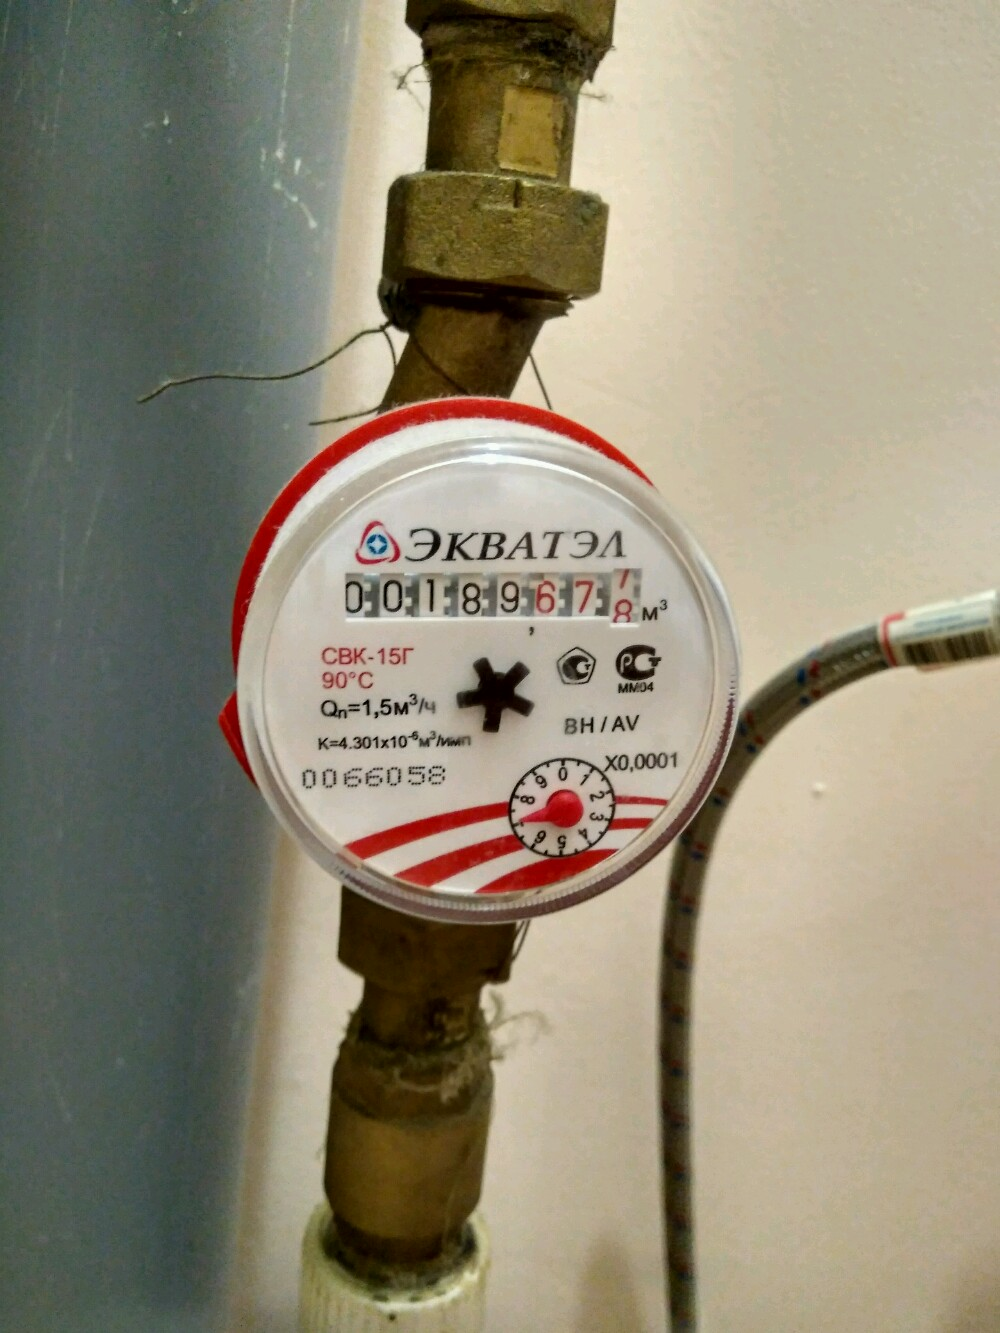
\includegraphics[width=0.84\linewidth]{assets/apresentacao/Img_Original_Unet.jpg}%
    }{%
      \begin{tikzpicture}
        \draw[draw=senacblue, fill=senacblue!5, rounded corners=3pt, thick] (0,0) rectangle (4.3,2.4);
        \node[align=center, font=\scriptsize\color{senacblue}] at (2.15,1.55) {\textbf{Bancada Experimental}\\ESP32-CAM + RD49C};
        \draw[draw=senacorange, thick, fill=white] (0.7,0.5) rectangle (3.6,1.05);
        \node[font=\ttfamily\footnotesize\bfseries, color=black!80] at (2.15,0.78) {0 0 0 0 2 5};
      \end{tikzpicture}%
    }\\[2pt]
    {\tiny Ilustração: Hidrômetro}
    {\tiny Fonte: Kucev  (2020)}
  \end{columns}

  \vspace{0.15cm}
  \begin{block}{Pergunta de pesquisa}
    \scriptsize De que maneira a adoção de processamento em borda ou em nuvem impacta eficiência energética, acurácia, complexidade de desenvolvimento de firmware e desempenho computacional em \textit{smart metering} via LoRaWAN?
  \end{block}
\end{frame}

% ===============================================================
\section{Objetivos}
% ===============================================================
\begin{frame}{Objetivos}
  \begin{block}{Objetivo geral}
    \footnotesize Comparar viabilidade técnica, acurácia e consumo energético entre OCR local no \textbf{ESP32-CAM} (\textit{Edge}) e OCR remoto em \textbf{servidor} (\textit{Cloud}) sobre rede \textbf{LoRaWAN}.
  \end{block}
  \vspace{0.12cm}
  {\footnotesize\bfseries\color{senacblue}Objetivos específicos}
  \vspace{0.06cm}
  \footnotesize
  \renewcommand{\arraystretch}{1.25}
  \begin{tabular}{@{}r >{\raggedright\arraybackslash}p{12.5cm}@{}}
    \textbf{\color{senacorange}1} & Implementar os dois fluxos: \textit{Edge} (OCR local no ESP32-CAM) e \textit{Cloud} (envio da imagem ao servidor). \\
    \textbf{\color{senacorange}2} & Configurar o enlace LoRaWAN AU915 (Ato n\textordmasculine~14.448/ANATEL) e o repouso do nó entre leituras para reduzir corrente em repouso (mA). \\
    \textbf{\color{senacorange}3} & Avaliar e comparar precisão de leitura (\%), latência (ms), consumo (mAh/leitura) e volume (bytes/leitura), identificando o \textit{trade-off}. \\
  \end{tabular}
\end{frame}

% ===============================================================
\section{Hipótese}
% ===============================================================
\begin{frame}{Hipóteses}
  \centering
  \begin{tikzpicture}[
      cartao/.style={draw=senacblue, rounded corners=4pt, fill=senacblue!5, inner sep=5pt,
                     anchor=north}]
    \node[cartao] at (0,0) {\begin{minipage}[t][3.6cm][t]{4.0cm}\raggedright
      {\normalsize\bfseries\color{senacorange}H1 --- Quantização}\\[3pt]
      {\scriptsize A quantização INT8 aplicada ao classificador causa redução de acurácia em comparação à versão FP32.}\end{minipage}};
    \node[cartao] at (4.75,0) {\begin{minipage}[t][3.6cm][t]{4.0cm}\raggedright
      {\normalsize\bfseries\color{senacorange}H2 --- Custo no Nó}\\[3pt]
      {\scriptsize O processamento local apresenta custo computacional maior no dispositivo final do que o remoto.}\end{minipage}};
    \node[cartao] at (9.5,0) {\begin{minipage}[t][3.6cm][t]{4.0cm}\raggedright
      {\normalsize\bfseries\color{senacorange}H3 --- Energia}\\[3pt]
      {\scriptsize A abordagem em nuvem apresenta autonomia energética inferior durante a transmissão em relação à borda.}\end{minipage}};
  \end{tikzpicture}

  \vspace{0.2cm}
  {\tiny\color{black!70}Métricas complementares avaliadas: latência de ponta a ponta (s), PDR por pacote e entrega por leitura (\%).}
\end{frame}

% ===============================================================
\section{Justificativa}
% ===============================================================
\begin{frame}{Justificativa}
  \begin{itemize}\footnotesize
    \setlength{\itemsep}{4pt}
    \item \textbf{Lacuna empírica}: carência de comparações controladas entre borda e nuvem sobre o mesmo hardware e enlace (Andriulo et al., 2024).
    \item \textbf{Economia com \textit{retrofitting}}: viabiliza digitalização de medidores analógicos existentes sem substituição física completa.
    \item \textbf{Desafios técnicos}:
      \begin{itemize}\scriptsize
        \item executar inferência de visão computacional em hardware com PSRAM limitada (4 MB);
        \item transmitir imagem comprimida em JPEG fragmentada em múltiplos pacotes via LoRaWAN de baixa taxa.
      \end{itemize}
    \item \textbf{Insumos de projeto}: métricas quantitativas de energia, latência, acurácia para decisões arquiteturais.
  \end{itemize}
\end{frame}

% ===============================================================
\section{Metodologia bibliográfica}
% ===============================================================
\begin{frame}{Metodologia Bibliográfica}
  \centering
  \begin{tikzpicture}[
      bloco/.style={draw=senacblue, rounded corners=3pt, fill=senacblue!5,
                    text width=12.0cm, align=center, font=\scriptsize, inner sep=4pt},
      setinha/.style={-{Stealth}, thick, senacorange}]
    \node[bloco] (p1) at (0,0) {\textbf{1. Identificação (Funil)} \quad|\quad Google Scholar, MDPI e Intechopen \quad|\quad \textbf{120 artigos} analisados por título};
    \draw[setinha] (p1.south) -- ++(0,-0.2);
    \node[bloco] (p2) at (0,-1.1) {\textbf{2. Strings de busca (ST01--ST09)}: Redes, Contexto e Hardware/Software \quad|\quad Ex.: \texttt{"ESP32-CAM" AND "analog meter" AND "OCR"}};
    \draw[setinha] (p2.south) -- ++(0,-0.2);
    \node[bloco] (p3) at (0,-2.2) {\textbf{3. Triagem assistida}: ResearchRabbit e Gemini Deep Research na descoberta de conexões e triagem inicial};
    \draw[setinha] (p3.south) -- ++(0,-0.2);
    \node[bloco] (p4) at (0,-3.3) {\textbf{4. Seleção}: publicações de 2020--2026 com foco prático em telemetria (sem filtro de data para obras seminais)};
    \draw[setinha] (p4.south) -- ++(0,-0.2);
    \node[bloco] (p5) at (0,-4.4) {\textbf{5. Adições Posteriores}: Trabalhos seminais e trabalhos específicos a aspectos de desenvolvimento};
  \end{tikzpicture}
\end{frame}

% ===============================================================
\section{Referencial Teórico}
% ===============================================================
\subsection{LoRa e LoRaWAN}
\begin{frame}{Referencial Teórico: LoRa e LoRaWAN}
  \begin{columns}[t]
    \column{0.48\textwidth}
    {\footnotesize\bfseries\color{senacblue}Camada Física (LoRa)}
    \begin{itemize}\scriptsize
      \setlength{\itemsep}{3pt}
      \item Modulação por espalhamento espectral \textit{Chirp Spread Spectrum} (CSS) da Semtech: longo alcance e baixo consumo.
      \item Parâmetros principais:
        \begin{itemize}\tiny
          \item \textbf{BW}: largura de banda em kHz;
          \item \textbf{SF}: fator de espalhamento (alcance e taxa);
          \item \textbf{CR}: taxa de codificação para redundância/correção.
        \end{itemize}
    \end{itemize}
    \column{0.49\textwidth}
    {\footnotesize\bfseries\color{senacblue}Protocolo (LoRaWAN)}
    \begin{itemize}\scriptsize
      \setlength{\itemsep}{3pt}
      \item Rede LPWAN \textit{open-source} (LoRa Alliance): dispositivos finais, \textit{gateways}, servidores de rede e aplicação.
      \item Criptografia simétrica \textbf{AES}; ativação \textbf{OTAA} ou \textbf{ABP}.
      \item Classes: \textbf{A} (menor consumo), \textbf{B} (janelas agendadas) e \textbf{C} (recepção contínua).
    \end{itemize}
  \end{columns}
\end{frame}

\subsection{Restrições Regulatórias}
\begin{frame}{Referencial Teórico: Restrições Regulatórias}
  \begin{columns}[t]
    \column{0.51\textwidth}
    {\footnotesize\bfseries\color{senacblue}Ato n\textordmasculine~14.448 da ANATEL (AU915)}
    \begin{itemize}\scriptsize
      \setlength{\itemsep}{3pt}
      \item Faixa ISM de 915 a 928~MHz no plano AU915 (sem restrição de \textit{duty cycle}).
      \item \textbf{Salto em canais $<$250~kHz (125~kHz)}: ocupação média $\leq$ \textbf{0,4~s} em 14~s e $\geq$35 canais.
      \item \textbf{Item 10.3 (Modulação Digital)}: dispensa salto e limite por canal se:
        \begin{itemize}\tiny
          \item largura a 6~dB $\geq$ \textbf{500~kHz};
          \item potência de pico $\leq$ 1~W e densidade $\leq$ 8~dBm em 3~kHz.
        \end{itemize}
    \end{itemize}
    \column{0.46\textwidth}
    {\footnotesize\bfseries\color{senacblue}Configuração DR6}
    \begin{itemize}\scriptsize
      \setlength{\itemsep}{3pt}
      \item AU915 possui 64 canais de 125~kHz (0--63) e 8 de 500~kHz (64--71).
      \item \textbf{DR6 (SF8 / 500~kHz)}: 12.500~bit/s nominais e \textit{payload} até \textbf{222~bytes}.
      \item Permite canal fixo (915,9~MHz, canal 64) em conformidade com o item 10.3.
    \end{itemize}
  \end{columns}
\end{frame}

\subsection{OCR}
\begin{frame}{Referencial Teórico: OCR}
  \begin{columns}[t]
    \column{0.48\textwidth}
    {\footnotesize\bfseries\color{senacblue}Pipeline e CNNs}
    \begin{itemize}\scriptsize
      \setlength{\itemsep}{3pt}
      \item Converte imagens com texto/dígitos em dados estruturados.
      \item Etapas clássicas: pré-processamento, localização/segmentação (ROI), classificação e pós-processamento.
      \item \textbf{CNNs}: convolução (com escala de cinza reduzindo canais), \textit{max pooling} e camadas densas.
    \end{itemize}
    \column{0.49\textwidth}
    {\footnotesize\bfseries\color{senacblue}Segmentação, Sequência e Quantização}
    \begin{itemize}\scriptsize
      \setlength{\itemsep}{3pt}
      \item \textbf{U-Net}: \textit{encoder}, \textit{bottleneck}, \textit{decoder} e \textit{skip connections} com perda híbrida BCE + \textit{Dice loss}.
      \item \textbf{CRNN + CTC}: leitura sequencial; em microcontroladores, LSTMs têm custo e suporte limitados.
      \item \textbf{Quantização INT8 e QAT}: reduzem memória e aceleram inferência embarcada.
    \end{itemize}
  \end{columns}
\end{frame}

\subsection{Edge e Cloud Computing}
\begin{frame}{Referencial Teórico: Edge e Cloud Computing}
  \centering
  \scriptsize
  \renewcommand{\arraystretch}{1.3}
  \begin{tabular}{@{}l >{\raggedright\arraybackslash}p{5.4cm} >{\raggedright\arraybackslash}p{5.4cm}@{}}
    \toprule
    \textbf{Critério} & \textbf{\color{corBorda}Edge Computing (Borda)} & \textbf{\color{corNuvem}Cloud Computing (Nuvem)} \\
    \midrule
    \textbf{Processamento} & Local no dispositivo final (ESP32-CAM) & Remoto em servidor \\
    \textbf{Tráfego de rede} & Menor tráfego de mensagens (9 bytes) & Maior quantidade de pacotes (blocos JPEG) \\
    \textbf{Latência} & Menor latência na transmissão & Alta latência \\
    \textbf{Hardware} & Capacidade computacional e RAM/PSRAM limitadas & Maior poder computacional e escalabilidade \\
    \textbf{Firmware e gestão} & Maior complexidade no nó & Menor complexidade de firmware e manutenção centralizada \\
    \bottomrule
  \end{tabular}
  \fonteslide{Adaptado de Andriulo et al. (2024).}
\end{frame}

% ===============================================================
\section{Desenvolvimento}
% ===============================================================
\subsection{Metodologia de Pesquisa}
\begin{frame}{Metodologia de Pesquisa: Etapas e POCs}
  \begin{columns}[t]
    \column{0.48\textwidth}
    {\footnotesize\bfseries\color{senacblue}Delineamento}
    \begin{itemize}\scriptsize
      \item Pesquisa aplicada, experimental e comparativa no mesmo hardware e enlace.
    \end{itemize}
    \vspace{0.1cm}
    {\footnotesize\bfseries\color{senacblue}Provas de Conceito (1--2)}
    \begin{itemize}\scriptsize
      \item \textbf{POC 1}: Tesseract e EasyOCR falharam na linha em $160\times120$; recorte por dígito funcionou.
      \item \textbf{POC 2}: enlace RD49C $\rightarrow$ LoRa32 em AU915 DR6 (canal 64, 915,9~MHz).
    \end{itemize}
    \column{0.49\textwidth}
    {\footnotesize\bfseries\color{senacblue}Evolução das POCs (3--5)}
    \begin{itemize}\scriptsize
      \item \textbf{POC 3 (Cloud)}: JPEG (q90) em blocos de até 175~B + 6~B cabeçalho (FPort 1); OCR no servidor via LiteRT.
      \item \textbf{POC 4 (Edge)}: TFLite Micro (\texttt{esp-tflite-micro} 1.3.1), ROI calibrada e 9~B (FPort 2).
      \item \textbf{POC 5 (Integração)}: firmwares autônomos, \textit{power-down} da câmera, \textit{deep sleep} de 30~s e INA219 a 100~Hz.
    \end{itemize}
  \end{columns}
\end{frame}

\begin{frame}{Metodologia de Pesquisa: Fluxos Abandonados}
  \begin{columns}[t]
    \column{0.32\textwidth}
    {\scriptsize\bfseries\color{senacblue}1. Encoder-Decoder ($192\times192$)}
    \begin{itemize}\tiny
      \setlength{\itemsep}{2pt}
      \item Localização automática na borda atingiu \textbf{15,5~s} ($\approx$17,6~s no ciclo) e \textbf{Dice 0,39}.
      \item Custo temporal e baixa precisão de segmentação inviabilizaram o uso contínuo.
    \end{itemize}
    \etiqueta{corFalha}{ABANDONADO}

    \column{0.32\textwidth}
    {\scriptsize\bfseries\color{senacblue}2. U-Net + CRNN + CTC}
    \begin{itemize}\tiny
      \setlength{\itemsep}{2pt}
      \item Servidor (30 fotos): \textbf{86,67\%} (26/30) de sequência completa e \textbf{94,58\%} por dígito.
      \item \textbf{Descartado no nó}:
        \begin{itemize}\tiny
          \item U-Net $384\times384$ exigiu \textbf{15.335.424~B} ($\approx$15,3~MB) contra 4~MB de PSRAM;
          \item operador \texttt{REDUCE\_PROD} ausente no Arduino-ESP32 3.0.7;
          \item U-Net compacta ($160\times160$, $\approx$1,7~MB) gerou máscara vazia em $\approx$15\%.
        \end{itemize}
    \end{itemize}
    \etiqueta{corFalha}{ABANDONADO}

    \column{0.33\textwidth}
    {\scriptsize\bfseries\color{senacblue}3. U-Net + CNN de Dígito ($68\times68$)}
    \begin{itemize}\tiny
      \setlength{\itemsep}{2pt}
      \item Herdou a limitação de memória da U-Net para execução embarcada.
      \item Treinada com fontes genéricas (Kaggle), fora do domínio de hidrômetros.
    \end{itemize}
    \etiqueta{corFalha}{ABANDONADO}
    \vspace{0.12cm}
    \begin{block}{Solução adotada}
      \tiny CNN leve ($28\times28$, 81,5~KB INT8) treinada com recortes de roletes + ROI calibrada na instalação.
    \end{block}
  \end{columns}
\end{frame}

\begin{frame}{Metodologia de Pesquisa: Métricas Avaliadas}
  \centering
  \scriptsize
  \renewcommand{\arraystretch}{1.25}
  \begin{tabular}{@{}l >{\raggedright\arraybackslash}p{4.3cm} >{\raggedright\arraybackslash}p{6.8cm}@{}}
    \toprule
    \textbf{Dimensão} & \textbf{Métricas} & \textbf{Procedimento} \\
    \midrule
    \textbf{\color{senacorange}OCR (H1)} & Leitura exata, acerto por dígito, CER, Macro-F1, Dice e IoU
      & FP32 $\times$ INT8 (7.378 recortes, 1.894 imagens Word-Wheel e 30 fotos físicas); McNemar \\
    \textbf{\color{senacorange}Hardware (H2)} & Tempo (ms), CPU (\%), frequência, pico de PSRAM (KB)
      & 30 ciclos instrumentados/fluxo (ROI + classe A) e 33 quadros no firmware de borda \\
    \textbf{\color{senacorange}Energia (H3)} & Carga (mAh), corrente (mA), autonomia (dias)
      & INA219 (shunt 0,1~$\Omega$, 100~Hz, 29 ciclos/fluxo); bateria ideal de 2.000~mAh \\
    \textbf{\color{senacorange}Rede (Compl.)} & Latência ponta a ponta (s), PDR e entrega por leitura (\%)
      & Seriais sincronizadas no PC (30 disparos/fluxo nos testes finais); teste exato de Fisher \\
    \bottomrule
  \end{tabular}
\end{frame}

\subsection{Implementação do Fluxo Definitivo}
\begin{frame}[fragile]{Implementação do Fluxo Definitivo: Arquitetura}
  \vspace{-0.4cm}
  \centering
  \makebox[\linewidth][c]{%
    \resizebox{0.70\textwidth}{!}{%
      \begin{tikzpicture}[
          font=\tiny,
          node distance=3.2mm and 3.5mm,
          bloco/.style={draw, rounded corners=2pt, align=center, fill=white,
                       minimum height=5.5mm, text width=#1},
          bloco/.default=4.8cm,
          seta/.style={-{Stealth[length=1.5mm]}, thick},
          rotulo/.style={font=\tiny\itshape, align=center}
      ]
          \node[bloco] (hidro) {Medidor analógico (mostrador de roletes)};
          \node[bloco, below=of hidro] (cam)
              {\textbf{ESP32-CAM}\\captura quadro $160\times120$ em tons de cinza e desliga câmera/\textit{deep sleep}};
          \node[bloco=4.2cm, draw=corBorda] (borda) at ($(cam.south)+(-2.35cm,-0.85cm)$)
              {\textbf{\color{corBorda}Fluxo em borda}\\classifica dígitos na ROI calibrada (TFLite Micro, INT8)\\envia leitura: \textbf{9 bytes, 1 pacote (FPort 2)}};
          \node[bloco=4.2cm, draw=corNuvem] (nuvem) at ($(cam.south)+(2.35cm,-0.85cm)$)
              {\textbf{\color{corNuvem}Fluxo em nuvem}\\comprime em JPEG (qualidade 90, 2,9--3,4~KB)\\envia blocos de até 175~B + 6~B cabeçalho (FPort 1)};
          \node[bloco] (radio) at ($(borda.south)!0.5!(nuvem.south)+(0,-7mm)$)
              {\textbf{Radioenge RD49C}\\módulo LoRaWAN por UART (comandos AT), classe A};
          \node[draw, dashed, rounded corners=3pt, inner sep=1.6mm,
                fit=(cam) (borda) (nuvem) (radio),
                label={[font=\tiny\bfseries, anchor=north west]north west:Nó sensor}] {};
          \node[bloco, below=6.5mm of radio] (rx)
              {\textbf{Receptor LoRa32}\\escuta canal 915,9~MHz e repassa quadros via serial};
          \node[bloco, below=of rx] (pc)
              {\textbf{Computador (servidor)}\\descriptografa (\texttt{AppSKey}); lê FPort 2 ou remonta JPEG e executa OCR via LiteRT (FPort 1)};
          \draw[seta] (hidro) -- (cam);
          \draw[seta] (cam.south) -- ++(0,-1.5mm) -| (borda.north);
          \draw[seta] (cam.south) -- ++(0,-1.5mm) -| (nuvem.north);
          \draw[thick] (borda.south) |- ([yshift=2.2mm]radio.north);
          \draw[thick] (nuvem.south) |- ([yshift=2.2mm]radio.north);
          \draw[seta] ([yshift=2.2mm]radio.north) -- (radio.north);
          \draw[seta] (radio) -- node[rotulo, right=1mm]
              {AU915, DR6 (SF8 / 500~kHz), canal 64 fixo, ABP} (rx);
          \draw[seta] (rx) -- node[rotulo, right=1mm] {USB-serial} (pc);
      \end{tikzpicture}%
    }%
  }
\end{frame}

\begin{frame}{Implementação: Hardware, Enlace e OCR}
  \begin{columns}[t]
    \column{0.48\textwidth}
    {\footnotesize\bfseries\color{senacblue}Hardware e Enlace}
    \begin{itemize}\scriptsize
      \setlength{\itemsep}{3pt}
      \item \textbf{Nó}: AI-Thinker ESP32-CAM (240~MHz, 4~MB PSRAM) + Radioenge RD49C; \textit{power-down} da câmera após captura.
      \item \textbf{Rede}: AU915, canal 64 (915,9~MHz), \textbf{DR6 (SF8 / 500~kHz)}, CR 4/5, +20~dBm, ABP, \textbf{Classe A}.
      \item \textbf{Tráfego}: \textbf{9~B} (1 pacote, $\approx$25,7~ms no ar) na borda $\times$ \textbf{2,9--3,4~KB} (17--20 pacotes nos testes finais) na nuvem.
    \end{itemize}
    \column{0.49\textwidth}
    {\footnotesize\bfseries\color{senacblue}Pipeline OCR e ROI}
    \begin{itemize}\scriptsize
      \setlength{\itemsep}{3pt}
      \item \textbf{CNN}: entrada $28\times28$ em cinza (72.442 parâmetros; \textbf{81,5~KB} em INT8 pós-treinamento).
      \item \textbf{Treino em 2 fases}: 49.038 recortes públicos (41.660 treino / 7.378 validação) + 24 recortes do ESP32-CAM.
      \item \textbf{ROI calibrada}: salva na flash do nó com recorte da \textbf{face do rolete} (14\%--74\% da largura).
    \end{itemize}
  \end{columns}
\end{frame}

\subsection{Resultados Alcançados}
\begin{frame}{Resultados: H1 --- Quantização INT8}
  \begin{columns}[c]
    \column{0.52\textwidth}
    \centering
    \begin{tikzpicture}
      \begin{axis}[estiloSlides, ybar, width=\linewidth, height=4.6cm,
          bar width=1.0cm, ymin=90, ymax=97, enlarge x limits=0.6,
          symbolic x coords={Float32,INT8}, xtick=data,
          ylabel={Acerto por dígito (\%)},
          nodes near coords, nodes near coords style={font=\footnotesize\bfseries},
          point meta=explicit symbolic]
        \addplot[fill=senacblue!70, draw=none] coordinates {(Float32,95.46) [95,46] (INT8,95.38) [95,38]};
      \end{axis}
    \end{tikzpicture}\\
    {\tiny 7.378 recortes de validação}
    \column{0.45\textwidth}
    \begin{itemize}\scriptsize
      \item Diferença de \textbf{0,08 p.p.} (7.043 $\times$ 7.037 acertos; McNemar $p = 0{,}29$).
      \item Macro-F1: 0,946 (FP32) $\times$ 0,945 (INT8).
      \item Word-Wheel (1.894 imgs): \textbf{92,8\%} leitura exata e \textbf{97,7\%} dígito (CER 0,023).
      \item Hidrômetro físico (30 fotos): \textbf{25/30} (83,3\%) e 175/180 dígitos (97,2\%, CER 0,028) em ambas ($p = 1{,}0$).
    \end{itemize}
    \vspace{0.1cm}
    \etiqueta{senacorange}{REDUÇÃO DESPREZÍVEL}
  \end{columns}
\end{frame}

\begin{frame}{Resultados: Leitura de Ponta a Ponta}
  \begin{columns}[c]
    \column{0.58\textwidth}
    \centering
    \begin{tikzpicture}
      \begin{axis}[estiloSlides, xbar, scale only axis, width=4.2cm, height=3.9cm,
          bar width=0.4cm, xmin=0, xmax=112, xtick={0,20,40,60,80,100}, enlarge y limits=0.14,
          symbolic y coords={fis,man2,man,prev}, ytick={fis,man2,man,prev},
          yticklabels={{Físico: ROI + face},{Comum: endireitada},{Comum: ROI manual},{Comum: prevista}},
          y dir=reverse, yticklabel style={font=\tiny, align=right},
          xlabel={Leituras exatas (\%)},
          nodes near coords, nodes near coords style={font=\scriptsize\bfseries, anchor=west},
          point meta=explicit symbolic]
        \addplot[fill=senacblue!70, draw=none, bar shift=0pt]
          coordinates {(0,prev) [0\%] (46,man) [46\%] (82,man2) [82\%] (83,fis) [83\%]};
      \end{axis}
    \end{tikzpicture}
    \column{0.39\textwidth}
    \begin{itemize}\scriptsize
      \item \textbf{Comum (39 fotos)}: 46\% leituras (85\% dígitos) com janela manual; \textbf{82\%} leituras (92\% dígitos) endireitada no servidor.
      \item \textbf{Físico bancada (30 fotos)}: ROI + face atingiu \textbf{83\%} (25/30) leituras e \textbf{97\%} (175/180) dígitos.
      \item JPEG q90 \textbf{não alterou} os acertos entre borda e nuvem.
    \end{itemize}
  \end{columns}
  \fonteslide{Placa e servidor produziram leituras idênticas nos 33 quadros da bancada enviados à placa.}
\end{frame}

\begin{frame}{Resultados: H2 --- Custo Computacional e Latência}
  \begin{columns}[c]
    \column{0.57\textwidth}
    \centering
    \begin{tikzpicture}
      \begin{axis}[estiloSlides, xbar, xmode=log, log basis x=10, log origin=infty,
          scale only axis, width=3.9cm, height=3.5cm, bar width=0.38cm, enlarge y limits=0.16,
          xmin=1, xmax=1000000, xtick={1,100,10000,1000000},
          xticklabels={1,100,{10.000},{1.000.000}},
          xlabel={Tempo por leitura (ms, escala log.)},
          symbolic y coords={srv,jpeg,roi,loc}, ytick={srv,jpeg,roi,loc}, y dir=reverse,
          yticklabels={{Servidor: 6 dígitos},{Nuvem: comp. JPEG},{Borda: 6 dígitos (ROI)},{Borda: loc. inicial}},
          yticklabel style={font=\tiny, align=right},
          nodes near coords, point meta=explicit symbolic,
          nodes near coords style={font=\scriptsize, anchor=west}]
        \addplot[fill=corNuvem!45, draw=none, bar shift=0pt] coordinates {(1.91,srv) [1,91~ms]};
        \addplot[fill=corNuvem, draw=none, bar shift=0pt] coordinates {(11,jpeg) [11~ms]};
        \addplot[fill=corBorda, draw=none, bar shift=0pt] coordinates {(1917,roi) [1.917~ms]};
        \addplot[fill=corBorda!45, draw=none, bar shift=0pt] coordinates {(17568,loc) [17.568~ms]};
      \end{axis}
    \end{tikzpicture}
    \column{0.40\textwidth}
    \begin{itemize}\scriptsize
      \item \textbf{Nó (H2)}: 1.917~ms (100\% núcleo 1) e \textbf{788,9~KB} PSRAM na borda $\times$ 11~ms e \textbf{148,9~KB} na nuvem (240~MHz). \etiqueta{corOk}{H2 CONFIRMADA}
      \item \textbf{Latência ponta a ponta}: \textbf{3,50~s} (borda) $\times$ \textbf{148,3~s} (nuvem, classe A) --- borda $\approx$42$\times$ mais rápida.
      \item \textbf{Entrega (classe A)}: 96,7\% (29/30) borda $\times$ 80,0\% (24/30) nuvem ($p = 0{,}10$).
    \end{itemize}
  \end{columns}
\end{frame}

\begin{frame}{Resultados: H3 --- Energia e Autonomia}
  \begin{columns}[c]
    \column{0.6\textwidth}
    \centering
    \scriptsize
    \renewcommand{\arraystretch}{1.15}
    \begin{tabular}{@{}lrr@{}}
      \toprule
      & \textbf{\color{corNuvem}Nuvem} & \textbf{\color{corBorda}Borda} \\
      \midrule
      \multicolumn{3}{@{}l}{\textit{Testes iniciais (27/10): localização automática, classe C}} \\
      Carga por leitura & 4,64~mAh & 0,824~mAh \\
      Corrente em repouso & 23,7~mA & 25,2~mA \\
      \addlinespace
      \multicolumn{3}{@{}l}{\textit{Testes finais (19/11): ROI calibrada, classe A (adotada)}} \\
      Carga por leitura (média) & \textbf{2,91~mAh} & \textbf{0,175~mAh} \\
      Corrente em repouso & 6,3~mA & 6,1~mA \\
      Autonomia (1 leit./10~min) & 3,8 dias & \textbf{12,1 dias} \\
      Autonomia (1 leit./hora) & 9,5 dias & \textbf{13,2 dias} \\
      \bottomrule
    \end{tabular}\\[2pt]
    {\tiny Modelo ideal para bateria hipotética de 2.000~mAh; repouso de 30~s nas medições}
    \column{0.37\textwidth}
    \bignum[corBorda]{16,7$\times$}{menos carga por leitura na borda}
    \vspace{0.1cm}
    \begin{itemize}\scriptsize
      \item Consumo regido pelo \textbf{tempo acordado} (147,6~s $\times$ 6,49~s).
      \item \textbf{Classe A} reduziu o repouso de $\approx$24 para $\approx$6,2~mA.
    \end{itemize}
    \etiqueta{corOk}{H3 CONFIRMADA}
  \end{columns}
\end{frame}

\subsection{Retomada dos Objetivos}
\begin{frame}{Retomada dos Objetivos e Hipóteses}
  \begin{block}{Resposta à Pergunta de Pesquisa}
    \scriptsize Em enlaces LoRaWAN de baixa taxa, o \textbf{volume de dados transmitido pesa mais que a capacidade de processamento}: enviar 9~B em vez de $\approx$4~KB tornou a borda $\approx$42$\times$ mais rápida e 16,7$\times$ mais econômica por leitura, sem perda prática de acurácia.
  \end{block}
  \vspace{0.08cm}
  \begin{itemize}\scriptsize
    \setlength{\itemsep}{2.5pt}
    \item \textbf{Objetivo Geral}: atingido --- borda e nuvem comparadas empiricamente no mesmo hardware.
    \item \textbf{OE1 (Fluxos)}: atingido --- firmwares autônomos com \textit{deep sleep} implementados no mesmo hardware.
    \item \textbf{OE2 (Enlace e Repouso)}: atingido \textbf{em parte} --- AU915 DR6 e Classe A baixaram o repouso para $\approx$6~mA, ainda dominante em intervalos longos.
    \item \textbf{OE3 (Métricas)}: atingido --- \textbf{H1} com efeito desprezível; \textbf{H2} e \textbf{H3} confirmadas.
  \end{itemize}
\end{frame}

\subsection{Contribuição para a Computação}
\begin{frame}{Contribuição para a Computação}
  \begin{itemize}\scriptsize
    \setlength{\itemsep}{4pt}
    \item \textbf{Benchmark controlado}: comparação direta \textit{Edge} $\times$ \textit{Cloud} sobre o mesmo hardware, modelos e enlace LoRaWAN.
    \item \textbf{Três diretrizes para projetos IoT de baixa taxa}:
      \begin{enumerate}\scriptsize
        \item volume transmitido domina latência e consumo por leitura mais que a velocidade de inferência;
        \item ganho de autonomia na borda depende da redução da corrente em repouso (Classe A);
        \item precisão da ROI e recorte da face da roda importam mais que a arquitetura ou quantização INT8.
      \end{enumerate}
    \item \textbf{Conformidade regulatória}: envio de blocos de imagem em canal fixo de 500~kHz no AU915 (item 10.3/ANATEL).
    \item \textbf{Reprodutibilidade}: firmwares, calibrador de ROI, \textit{scripts} e dados de medição em repositório público.
  \end{itemize}
\end{frame}

\subsection{Limitações}
\begin{frame}{Limitações e Trabalhos Futuros}
  \begin{columns}[t]
    \column{0.48\textwidth}
    {\footnotesize\bfseries\color{senacblue}Limitações}
    \begin{itemize}\scriptsize
      \setlength{\itemsep}{2.5pt}
      \item Conjunto comum e calibração em monitor; 30 fotos em 1 hidrômetro físico com iluminação fixa.
      \item Enlace de bancada: 1 nó, receptor monocanal (sem \textit{gateway} multicanal), sem retransmissão e RSSI de $-60$ a $-49$~dBm.
      \item Alimentação por USB (5~V); $\approx$6~mA em repouso não separados entre rádio e placa; autonomia ideal.
      \item Disparo marcado 0,3--0,5~s após o despertar real; latência na nuvem sem OCR no servidor ($\approx$2~ms).
    \end{itemize}
    \column{0.48\textwidth}
    {\footnotesize\bfseries\color{senacblue}Trabalhos Futuros}
    \begin{itemize}\scriptsize
      \setlength{\itemsep}{2.5pt}
      \item Avaliar múltiplos hidrômetros e iluminações, além de roletes em transição.
      \item Testar em campo com \textit{gateway} multicanal, múltiplos nós e retransmissão seletiva de blocos.
      \item Investigar a causa dos 15,6~s do modelo de localização no microcontrolador.
      \item Avaliar U-Net + CRNN + CTC em hardware/versão compatível e implementar atualização OTA.
    \end{itemize}
  \end{columns}
\end{frame}

% ---------------------------------------------------------------
% ENCERRAMENTO
% ---------------------------------------------------------------
\begin{frame}[plain]
  \centering
  \vspace{1cm}
  \logosenacgrande

  \vspace{0.7cm}
  {\Large\bfseries\color{senacblue}Obrigado!\par}
  \vspace{0.25cm}
  {\normalsize Perguntas?\par}
\end{frame}

% ---------------------------------------------------------------
% APÊNDICE
% ---------------------------------------------------------------
\appendix

\begin{frame}{Apoio - Corrente do Nó em um Ciclo (Classe A)}
  \centering
  \begin{tikzpicture}
    \begin{groupplot}[estiloSlides,
        group style={group size=1 by 2, vertical sep=1.15cm},
        width=0.95\textwidth, height=2.9cm,
        xmin=0, xmax=175, ymin=0, ymax=250, ytick={0,100,200},
        ylabel={mA}]
      \nextgroupplot[title={\color{corNuvem}Nuvem: ciclo de 171~s, 2,88~mAh (média de 2,91~mAh)}]
      \IfFileExists{sections/dados/corrente_ciclo_nuvem_classe_a.dat}{%
        \addplot[color=corNuvem, line width=0.35pt] table {sections/dados/corrente_ciclo_nuvem_classe_a.dat};
      }{%
        \addplot[color=corNuvem, line width=0.8pt] coordinates {
          (0,6.3) (0.2,145) (1.5,185) (2.0,65) (10,72) (30,68) (60,75) (90,69) (120,74) (147.6,70) (148.0,6.3) (171,6.3)
        };
      }
      \nextgroupplot[title={\color{corBorda}Borda: ciclo de 34~s, 0,176~mAh (média de 0,175~mAh)},
                     xlabel={Tempo desde o despertar (s)}]
      \IfFileExists{sections/dados/corrente_ciclo_borda_classe_a.dat}{%
        \addplot[color=corBorda, line width=0.35pt] table {sections/dados/corrente_ciclo_borda_classe_a.dat};
      }{%
        \addplot[color=corBorda, line width=0.8pt] coordinates {
          (0,6.1) (0.2,145) (1.2,180) (1.6,95) (3.5,98) (4.5,130) (6.49,68) (6.8,6.1) (34,6.1)
        };
      }
    \end{groupplot}
  \end{tikzpicture}
  \fonteslide{ROI calibrada e rádio em classe A, repouso de 30~s (testes finais). Envelope mín./máx. a cada 0,25~s (100~Hz).}
\end{frame}

\begin{frame}{Apoio - Precisão Exigida da ROI}
  \begin{columns}[c]
    \column{0.6\textwidth}
    \centering
    \begin{tikzpicture}
      \begin{axis}[estiloSlides, width=\linewidth, height=4.9cm,
          xmin=-0.3, xmax=6.3, ymin=0, ymax=100,
          xtick={0,1,2,3,4,6}, xticklabels={0,$\pm$1,$\pm$2,$\pm$3,$\pm$4,$\pm$6},
          xlabel={Erro máximo sorteado em cada coordenada da ROI (pixels)},
          ylabel={Leituras exatas (\%)}, legend pos=south west]
        \addplot[color=senacblue, line width=1pt, mark=*, mark size=1.6pt]
          coordinates {(0,82) (1,71) (2,62) (3,51) (4,40) (6,20)};
        \addlegendentry{Fatias iguais}
        \addplot[color=senacorange, line width=1pt, mark=square*, mark size=1.5pt, densely dashed, mark options={solid}]
          coordinates {(0,87) (1,81) (2,70) (3,64) (4,50) (6,26)};
        \addlegendentry{Votação entre 5 caixas}
      \end{axis}
    \end{tikzpicture}
    \column{0.37\textwidth}
    \begin{itemize}\scriptsize
      \item Cada dígito tem $\approx$16~px de largura: $\pm$2~px já deslocam 1/8 do dígito.
      \item Votação compensa $\approx$1~px ao custo de 5 inferências no servidor.
      \item Câmera fixa preservou a ROI entre leituras no medidor da bancada.
    \end{itemize}
  \end{columns}
  \fonteslide{Conjunto comum, fluxo em nuvem, quadro endireitado.}
\end{frame}

\begin{frame}{Apoio - Memória do TensorFlow Lite Micro}
  \centering
  \scriptsize
  \renewcommand{\arraystretch}{1.2}
  \begin{tabular}{@{}lrr@{}}
    \toprule
    \textbf{Item} & \textbf{Reservado (bytes)} & \textbf{Usado (bytes)} \\
    \midrule
    Buffer de quadro da câmera & --- & $\approx$19.216 \\
    Arena do classificador de dígitos & 786.432 & 28.556 \\
    \bottomrule
  \end{tabular}

  \vspace{0.3cm}
  \begin{itemize}\scriptsize
    \item Com ROI calibrada, apenas o classificador é carregado: pico de \textbf{788,9~KB} de PSRAM (modelo usa $<$29~KB).
    \item Firmware compilado ocupa 563~KB ($\approx$17\% da memória de programa); arena de 768~KB mostrou-se superdimensionada.
  \end{itemize}
\end{frame}

\begin{frame}{Apoio - Entrega dos Dados (PDR $\times$ Leitura)}
  \begin{columns}[c]
    \column{0.58\textwidth}
    \centering
    \begin{tikzpicture}
      \begin{axis}[estiloSlides, ybar, width=\linewidth, height=4.6cm,
          bar width=0.65cm, ymin=0, ymax=112, enlarge x limits=0.45,
          symbolic x coords={Pacotes,Leituras}, xtick=data,
          ylabel={Taxa de entrega (\%)},
          legend style={at={(0.5,1.02)}, anchor=south, legend columns=2},
          nodes near coords, nodes near coords style={font=\scriptsize\bfseries},
          point meta=explicit symbolic]
        \addplot[fill=corNuvem, draw=none] coordinates {(Pacotes,98.9) [98,9] (Leituras,80.0) [80,0]};
        \addplot[fill=corBorda, draw=none] coordinates {(Pacotes,96.7) [96,7] (Leituras,96.7) [96,7]};
        \legend{Nuvem, Borda}
      \end{axis}
    \end{tikzpicture}\\
    {\tiny Testes finais: ROI calibrada e rádio em classe A}
    \column{0.39\textwidth}
    \begin{itemize}\scriptsize
      \item Sem retransmissão no modo autônomo, 1 bloco perdido anula a imagem: 551/557 (98,9\%) PDR $\rightarrow$ 24/30 (80,0\%) leituras.
      \item Borda: 29/30 (96,7\%) por pacote e por leitura; Fisher $p = 0{,}10$.
      \item Nos testes iniciais (classe C), a entrega por leitura foi de 66,7\% (nuvem) e 79,4\% (borda).
    \end{itemize}
  \end{columns}
\end{frame}

\end{document}